\section{High-Level Compiler (WIP)} 

%To target spatial architectures, we use Spatial, an open source domain specific language for reconfigurable accelerators \cite{spatial_koeplinger}.
We use Spatial~\cite{spatial_koeplinger}--an domain specific language for reconfigurable
accelerators--as the front-end of Plasticine.
Spatial describes applications with imperative control constructs, such as loops and branches,
augmented with parallel patterns~\cite{parallelpattern}.
Parallel patterns are transformation functions on memory collections that capture both the access
patterns and the parallelization scheme of the operator.
Examples of popular parallel patterns include \emph{map} and \emph{reduce}.
Instead of software data-structures, spatial exposes hardware memories available on reconfigurable
hardware, such as registers and SRAM, directly to programmers.
These memory types allow user to explicitly control data transferring between different levels of
memory hierarchy to maximize locality.
Additionally, Spatial also includes important design parameters 
that are essential for achieving a good performance on a spatial architecture in the language
constructs.
Parameters include blocking size, loop unrolling factors, and pipelining schemes, which make it
easy to perform application-level design space exploration.
To enable loop-level parallelization and pipelining, Spatial automatically partitions and buffers 
intermediate on-chip memories.
An example of outer product---element-wise multiplication of two vectors resulting in a matrix---in Spatial is shown in Figure~\ref{fig:spatial_app}.
%In this example we assume inputs \emph{vecA}, \emph{vecB} and outputs \emph{matC} do not fit on chip.
%First, \emph{C2} and \emph{C4} load tiles of vectors of size \emph{tsA} and \emph{tsB} to on-chip scratchpads \emph{tileA} and \emph{tileB}. 
%Next, loop \emph{C5} computes the outer products and store it to scratchpad \emph{tileC}. 
%Finally, \emph{C6} stores partial results back to DRAM. 

\begin{figure}
\centering
  \begin{minipage}{0.6\textwidth}
\lstinputlisting[language=Spatial,linewidth=1\textwidth]{code/OuterProduct.scala}
  \end{minipage}
  \caption{Example of Outer Product in Spatial.}
\label{fig:spatial_app}
\end{figure}

\begin{figure*}
\centering
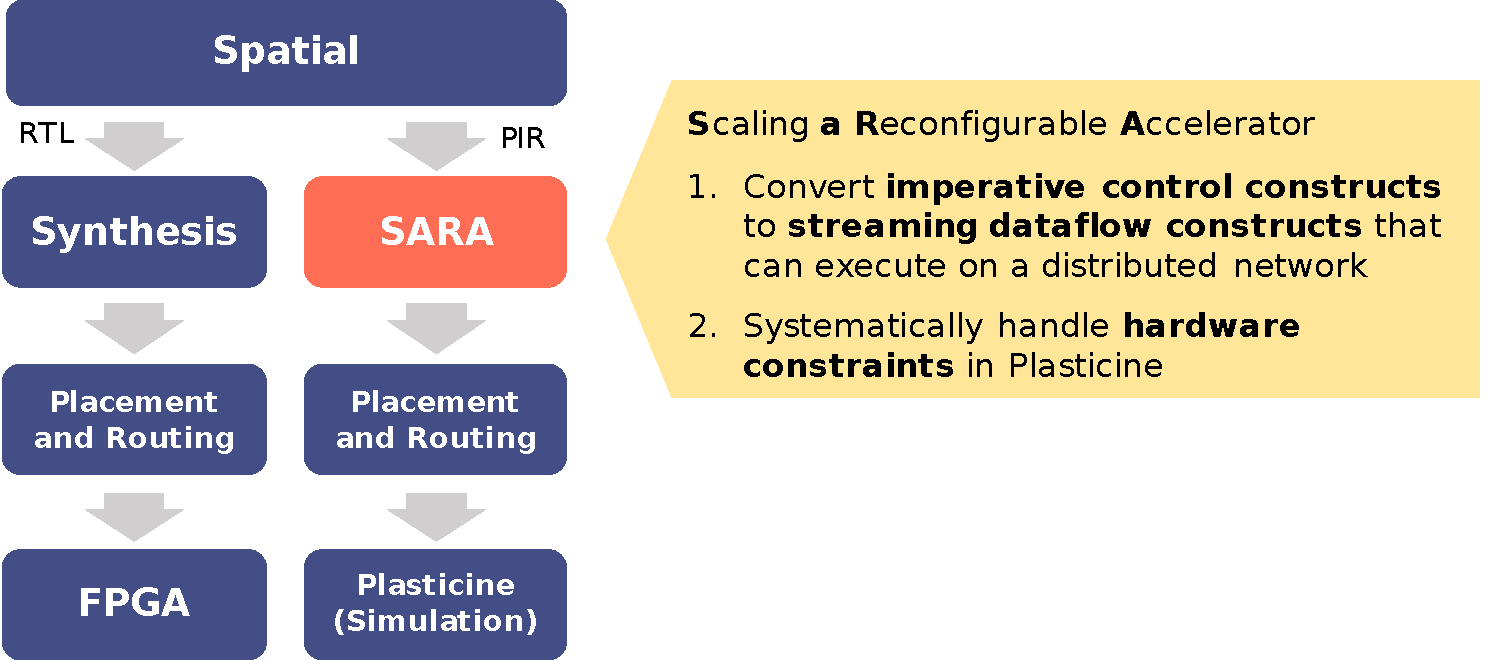
\includegraphics[width=1\textwidth]{figs/spatialstack.pdf}
\caption[Spatial compiler stack to target FPGAs and Plasticine]{
  Spatial compiler stack to target FPGAs and Plasticine
}
\label{fig:spatialstack}
\end{figure*}

Spatial is a target-agnostic language for general reconfigurable architectures. 
The primary targets of Spatial are FPGAs.
Similar to the c-based high-level synthesis tools, such as Vivado HLS~\cite{vivado} and
SDAccel~\cite{sdaccel},
Spatial provides a high-level programming interface that focuses on the algorithmic 
implementations of the application, hiding the hardware interfaces and low-level RTL programming from the
programmers.
To target Plasticine, we takes applications described in Spatial, disabling FPGA-specific
transformations, and perform architecture-specific lowering to \name's IR.
The key transformations we take from the Spatial compiler is loop unrolling and memory banking,
explained later in \Cref{sec:memsplit}.
Optimizations, such as retiming and scheduling, are disabled for Plasticine, as they cannot be
directly applied.
\Cref{fig:spatialstack} summarize the compiler flow to target FPGAs and Plasticine.

Although \name takes Spatial as front-end, the compilation techniques in \name can be equally
applied to other imperative languages with similar control constructs, such as C-based high-level
synthesis language, the backend of Halide IR, the TACO compiler, etc.
Using Spatial as our front-end language, however, has a few advantages.
Instead of adopting languages designed for processors to spatial accelerators like most HLS languages, 
Spatial is a language designed specifically for reconfigurable architectures.
Spatial's language constructs can capture the scheduling scheme that can be explored by most
spatial architectures, such as coarse-grained pipelining, streaming dataflow, hierarchical parallelization, 
finite state machines (FSM), without tying to a particular architecture.

%% Memory model
The data structure reprsented most exisitng imperative languages IR often marries to the
CPU's virtual memory model. LLVM-based compilers, for example, treats data collections as pointers to a shared
global address space, without distinguising what data are stored on-chip vs. off-chip.
This is CPU provides the memory abstraction that any data within the global address space 
can be equally accessed and the hardware implicitly manage the data movement between on and off-chip 
access by brining
Accelerators on the other hand, has explicitly managed on-chip scratchpads, that is not a cached
version of main memory data implicitly managed by the hardware.
The idea is to have the algorithm, which has better understanding of the data characteristics, to
explicitly control what data gets moved on and off-chip to maximize locality.
Other important static analysis in synthesis compilers, such as banking analysis, requires the
compiler to have the global view all access patterns on a data structure.
Therefore, modeling the data structures as disjoint memory space is much more suitable 
than pointers to a shared memory for reconfigurable architectures.

Most compilers for CPU uses a control flow graph to represent the control of a imperative program.
The control flow graph implicitly assumes the program is executed in time, which make it unsuitable
for analysis of a reconfigurable architecture that executes the program in space. 
Spatial uses a control hierarchy in the IR to captures the scheduling of the program.
The control hiearchy uses a tree structure to represent the nested control constructs, making it
easier to search the LCA of two controllers.
\Cref{fig:spatialegpar} shows an example of a control flow graph vs. a control hiearchy.
The controller at each level of the hierarchy corresponds to a control primitive, such as a loop, or
a branch statement. 
A basic block is attached to each \emph{innermost} controller including instructions
and memory accesses to user declared data-structures.
If the program has instructions in a outer loop, Spatial automatically inserts a \emph{unit}
controller to wrap the floating instructions.
\name takes the backend of Spatial IR as the input, which is an control hierarchy after loop
unrolling.

\begin{figure*}
\centering
\begin{subfigure}[b]{0.4\textwidth}
\inputminted{python}{code/spatialegpar.py}
\caption{Pseudo Spatial example}
\end{subfigure}
\hfill
\begin{subfigure}[b]{0.58\textwidth}
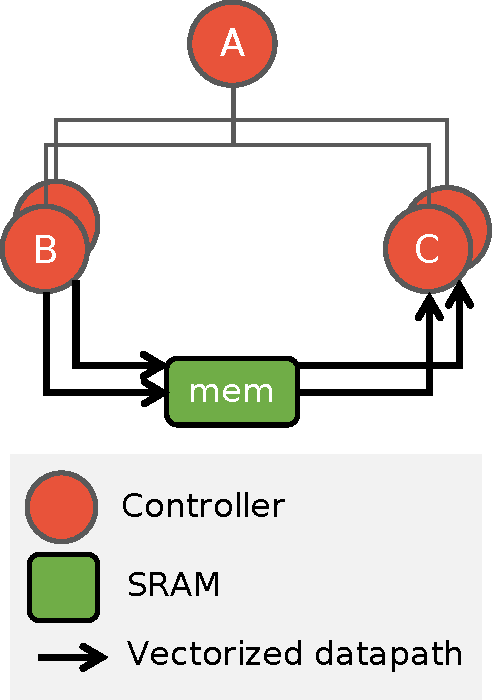
\includegraphics[width=1\textwidth]{figs/spatialir.pdf}
%\missingfigure[figwidth=1\textwidth]{Spatial IR}
\caption{Schematic Spatial IR}
\end{subfigure}
\caption[Spatial Example]{
  Pseudo example of \name's front-end language.
  (a) shows the an example of \name's front-end language. The actual front-end Spatial is a
  Scala-embedded DSL. For simplicity and generality, we use a python style pseudo code to show an
  language with similar abstraction. The `par` keyword indicates outer loop unrolling factor, and
  the `vec` keyword is followed by a inner-loop vectorization factor.
  When an iterator is vectorized, instructions using the vectorized iterator is automatically
  vectorized as well. When unrolling the outer loop \texttt{A}, the enclosed loop body and
  next-level control hierarchy are duplicated, as suggested in (b).
  Each loop in (a) corresponds to a controller in (b). The inner most controllers \texttt{B} and
  \texttt{C} each contain a basic block within instructions within the inner most loops.
}
\label{fig:spatialegpar}
\end{figure*}

Spatial is an embedded DSL in Scala.
For simplicity and generality, we will use python-style pseudo code to represents the front-end programming
abstraction for the rest of our discussion.
